%=====================================================================
\chapter{Fundamentação teórica}\label{chp:fund}
%========================================================

% \cite{isprs2021}       % (ISPRS, 2021)
% \citeonline{isprs2021} % ISPRS (2021)
% \citeauthor{isprs2021} % ISPRS
% \citeyear{isprs2021}   % 2021
% Exemplo de uma footnote\footnote{Para mais informações acesse \url{www.efoto.eng.uerj.br}}.

Este trabalho se propõe à análise da adoção de tecnologias da visão computacional em processos de fotogrametria, em especial, no software e-foto\footnote{Para mais informações acesse \url{www.efoto.eng.uerj.br}}. Por este motivo, as seções deste capítulo abordarão principalmente os conceitos de Fotogrametria e Visão Computacional.

\section{Fotogrametria}

% O que é a fotogrametria?
A fotogrametria é definida pela Sociedade Internacional para Fotogrametria e Sensoriamento Remoto (\textit{ISPRS – International Society for Photogrammetry and Remoto Sensing}) como ``a ciência e tecnologia de extrair informações geométricas e temáticas tridimensionais confiáveis, muitas vezes ao longo do tempo, de objetos e cenas a partir de imagens e dados espaciais''\cite{isprs2021}. Outra definição útil, como fizeram \citeauthoronline{coelho2007fotogrametria} (\citeyear{coelho2007fotogrametria}) em seu livro, é para o objetivo principal da fotogrametria, que pode ser enunciado como ``a reconstrução de um espaço tridimensional, chamado de espaço-objeto, a partir de um conjunto não vazio de imagens bidimensionais, chamado de espaço-imagem''. 

% Onde ela se aplica? 
Desde o advento da fotografia o estudo de sua aplicação para a documentação do espaço em que vivemos evoluiu bastante. Imediatamente foram descritos trabalhos para a documentação de edifícios e posteriormente, com o advento do avião, foram descritos métodos para fotografias aéreas. Modernamente, temos sensores em órbita da terra e de outros planetas, aeronaves leves não-tripuladas, além de sensores distintos do fotográfico como imageadores ativos ou sensores multi-espectrais.

Podemos então classificar a fotogrametria, numa primeira abordagem, segundo o ponto de vista das imagem utilizadas, a saber:

\begin{figure}[!ht]{12cm}
  \caption{Esquema de captação de imagens em aerolevantamentos.} \label{voo}
  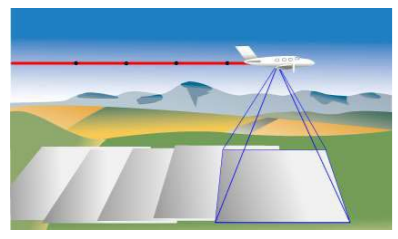
\includegraphics[width=\hsize]{figuras/voo.png}
  \source{Adaptado de \citeauthoronline{fricker2005pushbroom} (\citeyear{fricker2005pushbroom})}
\end{figure}

\begin{itemize}
    \item \textbf{Fotogrametria terrestre} que consiste na utilização das imagens primariamente geradas por sensores câmeras terrestres, ela é utilizada primariamente no campo da arquitetura, por exemplo, em restauração de fachadas históricas.
    \item \textbf{Fotogrametria aérea} também tratada como aerofotogrametria, se utiliza de imagens captadas por sensores ou câmaras a bordo de aeronaves, conforme ilustra a Figura \ref{voo}, e tem como produto resultante a reconstrução da superfície terrestre.
    \item \textbf{Fotogrametria orbital} compartilha inúmeras características com a aerofotogrametria, mas se distingue principalmente pelo uso de sensores orbitais, sendo capazes de observar uma porção maior de terreno numa única linha de varredura, com pequenas distorções.
\end{itemize}

% Qual é o fluxo de trabalho típico?
Estruturalmente, o processo de criação de produtos fotogramétricos pode ainda ser dividido em fases de trabalho bem definidas, como as que destacamos:

\begin{itemize}

    \item \textbf{Trabalho de planejamento:} onde ocorre a determinação do objeto ou região de estudo (espaço-objeto), são avaliadas informações locais, como acervos de dados pré-existentes e/ou são traçados planos para um novo imageamento.
    \item \textbf{Trabalho de campo:} onde é realizado o levantamento de pontos notáveis que sirvam como pontos de apoio de campo e/ou controle da qualidade, além do sobrevoo para capturar novas imagens, quando necessários.
    \item \textbf{Trabalho de laboratório:} onde são realizados o ajustamento para os parâmetros de orientação das imagens e a extração dos produtos desejados como modelos digitais de superfície, restituições tridimensionais ou ortomosaicos.
    
\end{itemize}

O ajustamento de parâmetros é fundamental para viabilizar todos os produtos que a fotogrametria pode gerar. Este ajustamento só é possível pela identificação de pontos do terreno no conjunto de imagens. Além desse fato, em grandes conjuntos de imagens provenientes de aerolevantamentos é mais eficiente ter pontos fotogramétricos, além dos pontos de controle, os quais representam o mesmo local do espaço objeto em imagens diferentes, sem que seja necessário o conhecimento prévio de suas coordenadas de mundo. São os pontos de controle que associam imagens ao terreno. Logo, estes são importantes para o ajuste absoluto do bloco de imagens. Por sua vez, os pontos fotogramétricos atuam como pontos de costura para um bloco de imagens seja ajustado relativamente.

\begin{figure}[!ht]{15cm}
  \caption{Reconstrução das coordenadas 3D a partir de imagens 2D.} \label{triang}
  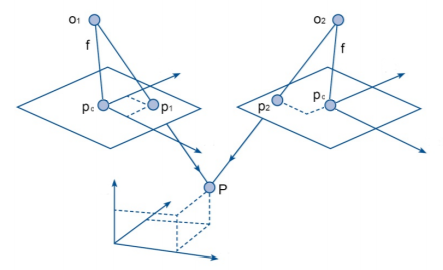
\includegraphics[width=\hsize]{figuras/triangulacao.png}
  \legend{$O_1$ e $O_2$ fornecem distintos valores $(X_0, Y_0, Z_0)$, pois são, expressos em 3D no sistema de referência do terreno assim como o ponto $P = (X,Y,Z)$. O termo $f$ é a distância focal da câmara usada na produção das imagens. Por sua vez, o ponto $p_c = (x_0, y_0)$ é o centro óptico da câmara expresso em 2D, pois está sobre espaço das imagens, assim como os pontos $p_{1}$ e $p_{2}$ com seus respectivos valores $(x, y)$.}
  \source{Adaptado de \url{https://ez-pdh.com/aerial-photogrammetry-help/}}
\end{figure}

Pontos fotogramétricos podem ainda ter suas coordenadas de mundo determinadas por consequência do ajustamento do bloco de imagens. A determinação destas coordenadas é possível pelo processo da triangulação espacial, ilustrado na Figura \ref{triang}, que pode ser derivado rearranjando os termos da Equação \ref{eqCol}, denominada equação de colinearidade. A triangulação de coordenadas 3D só é possível nas regiões de sobreposição imagens, pois é necessário obter ao menos duas observações no espaço das imagens a fim de atender o número de equações que permitam resolver o problema com 3 incógnitas (X, Y e Z).

\begin{equation} \label{eqCol}
    \begin{matrix} 
	x = x_0 - f 
	\frac{m_{11}(X - X_0) + m_{12}(Y - Y_0) + m_{13}(Z - Z_0)}
	     {m_{31}(X - X_0) + m_{32}(Y - Y_0) + m_{33}(Z - Z_0)} \\
	y = y_0 - f 
	\frac{m_{21}(X - X_0) + m_{22}(Y - Y_0) + m_{23}(Z - Z_0)}
	     {m_{31}(X - X_0) + m_{32}(Y - Y_0) + m_{33}(Z - Z_0)}
	\end{matrix}
\end{equation}

Os termos $m_{ij}$ na equação de colinearidade expressam a rotação entre os planos das imagens e os eixos do sistema de coordenadas adotado para o terreno, $(X_0, Y_0, Z_0)$ expressa a coordenada do ponto focal da lente da câmera no momento da captura da foto, $(x_0, y_0)$ expressa o ponto central das imagens registradas e $f$ expressa a distância focal do sistema sensor.


\subsection{A Estação Fotogramétrica Digital E-Foto}

% Quem desenvolveu o e-foto e quais são os seus motivadores?
Segundo seus desenvolvedores, o e-foto é uma iniciativa acadêmica de desenvolvimento de software livre para Fotogrametria Digital. Este é fruto principal do Projeto E-Foto, que é desenvolvido no Laboratório de Fotogrametria e Sensoriamento Remoto (LFSR) da Faculdade de Engenharia (FEN) da Universidade do Estado do Rio de Janeiro (UERJ), desde 2004. Através do software o projeto reduz as barreiras de custo para interessados em Fotogrametria \cite{EFotowebsite}. É importante também ressaltar sua relevância frente pacotes de softwares proprietários, em geral oferecidos em um modelo caixa preta, que revelam aos usuários pouquíssimos detalhes sobre os cálculos que são feitos, o que é aceitável para produção em larga escala, mas em um ambiente educacional tira a chance de inovação e de capacitação independente de plataformas por parte da comunidade estudantil.

% Quais as principais contribuições para sociedade?
Além do software o Projeto E-Foto possui outros desdobramentos significativos como o fomento para produção de diversos trabalhos de conclusão (como \citeauthoronline{correa2011} em \citeyear{correa2011}, \citeauthoronline{jonas2012} em \citeyear{jonas2012} e \citeauthoronline{regal2013} em \citeyear{regal2013}), incluindo este trabalho. São exemplos de produtos do projeto cursos, palestras, tutoriais (em texto e vídeo) e apresentações em fóruns nacionais e internacionais. Hoje o Projeto E-Foto é conhecido internacionalmente e atrai entusiastas do mundo inteiro tendo alguns produtos da comunidade usuária com o caso do livro produzido por \citeauthoronline{Martin_Vermeer2018} (\citeyear{Martin_Vermeer2018}).

% Como o software está dividido?
Entre os tutoriais para estudo do e-foto mais atuais é observada a subdivisão segundo os seguintes módulos com foco no trabalho laboratorial de um projeto fotogramétrico:
criação e gerenciamento de projetos (\textit{project creation and management}), 
orientação interior (\textit{interior orientation}),
orientação exterior por ressecção espacial (\textit{exterior orientation by space resection}),
fototriangulação por feixes perspectivos (\textit{exterior orientation by phototriangulation}),
restituição fotogramétrica 3D (\textit{Stereoplotter}),
extração do modelo digital de elevações (\textit{DSM Extraction}),
ortorretificação (\textit{Orthorectfication}) e
integração com o QGIS (\textit{Integration with QGIS}). 

% Quais destes módulos se destinam a fechar a inicialização do projeto?
Nos módulos de criação e gerenciamento de projetos, orientação interior, ressecção espacial e fototriangulação são realizadas atividades que têm por objetivo cadastrar, recuperar ou ajustar os parâmetros internos e externos ao sistema sensor durante o voo e obtenção do conjunto de imagens. São também fornecidos através destes módulos dados extras que possuem relevância para o processo, como sistema de referência adotado, características do sensor e do voo, pontos do terreno e suas medidas no conjunto de imagens que deve ser orientado. Num projeto com o e-foto o usuário só está apto a prosseguir aos demais módulos se todo o conjunto de imagens carregado recebeu parâmetros de orientação interior e exterior.

% Apresentar o fluxo de trabalho adaptado pelo aluno.
\begin{figure}[!ht]{14cm}
  \caption{Diagrama de atividades do e-foto} \label{fig:fluxo}
  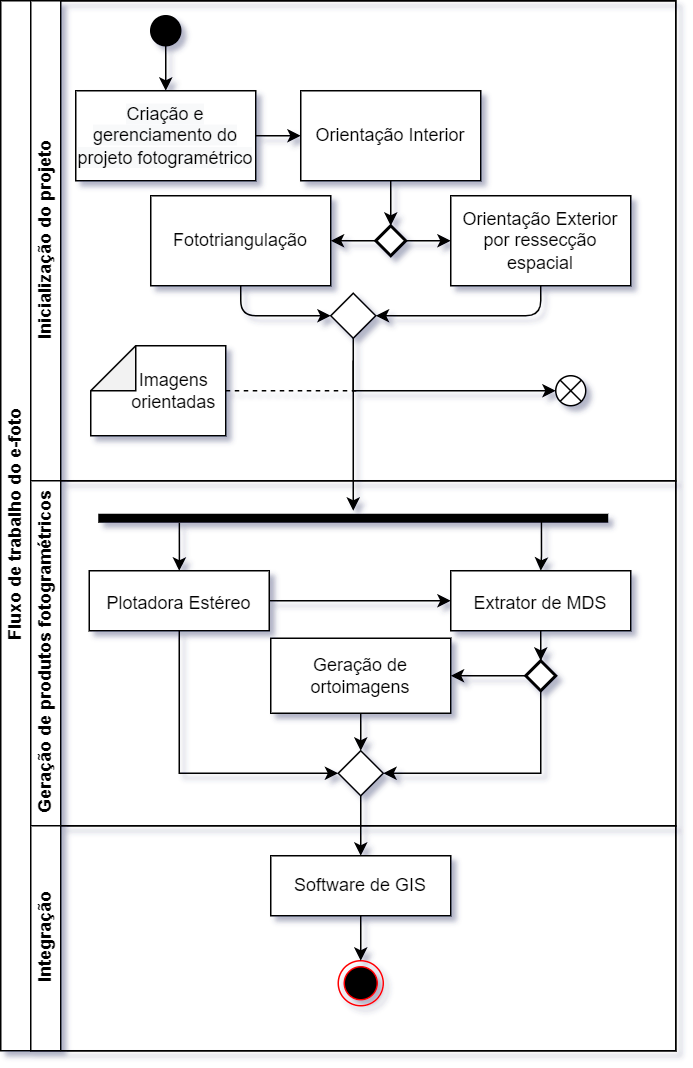
\includegraphics[width=\hsize]{figuras/Fluxograma_E-foto.png}
  %\legend{Texto da legenda.}
  \source{Adaptação de \url{http://www.efoto.eng.uerj.br/images/Documentos/0The_workflow_of_the_e-foto_software-16.06-v01.pdf}.}
\end{figure}

Está incluso no material de estudos um diagrama, similar ao adaptado pela Figura \ref{fig:fluxo}, de onde pode-se inferir que, apesar de cada módulo realizar possuir foco em atividades diferentes, alguns deles geram resultados análogos como, por exemplo, nos módulos de fototriangulação e de ressecção espacial, pois ambos podem ser utilizados em conjunto ou individualmente para finalizar a inicialização dos projetos, gerando os parâmetros de orientação exterior do bloco.

% Quais são os módulos que geram produtos fotogramétricos?
Além dos módulos referidos anteriormente há alguns outros que destinam-se a geração dos produtos fotogramétricos finais. Esses módulos se utilizam das imagens orientadas para criar diversos produtos como: restituição de vetores em 3D, modelos digitais de elevação (MDE) ou orto-mosaicos.

% Qual módulo se destaca nesse grupo para o presente trabalho e por que?
Por sua vez, o processo de medição de pontos homólogos, que preservaram as mesmas feições do terreno em distintas imagens, é realizado em diferentes módulos. Notavelmente isto ocorre tanto durante a atividades da fase de inicialização, como na geração de produtos finais. De modo geral a obtenção destas medidas é seguida pela interseção espacial que obtém as coordenadas 3D da feição no terreno. No entanto, deve ser destacado que estas medidas podem ser automatizadas, como no caso da extração de MDE, ou manuais, como no caso da restituição 3D e da fototriangulação. 

Em fato, alguma automação para obter estas medidas seria bem vinda em todas as etapas do software. Por tais motivos, vale destacar a função e estado de desenvolvimento de cada um destes módulos conforme segue:

\begin{description}
   \item[Fototriangulação]
   Este módulo permite o cálculo simultâneo dos parâmetros de orientação exterior do bloco de imagens num projeto. Isto requer que todas as imagens possuam orientação interior prévia. Ele oferece uma interface para visualização e medição de pontos de controle e fotogramétricos. Após a inserção do mínimo de pontos necessários, que depende do número de imagens no projeto, é habilitada a função de executar os cálculos de ajustamento do bloco. Com o ajustamento são obtidas as coordenadas geográficas de imagens e pontos fotogramétricos. Apesar de funcional, esse módulo ainda pode receber melhorias já previstas por seus autores, como a automação das medições de pontos fotogramétricos, a indicação de regiões de von gruber para orientar a medição de pontos fotogramétricos e a exclusão de pontos inseridos.
   \item[Restituição 3D] 
   Este módulo permite a visualização estereoscópica de pares de imagens previamente orientadas e a vetorização das feições observadas, isto é, produção de pontos, linhas e polígonos em 3D que possam ser transportados para outras aplicações de produção cartográfica, como o QGIS, pela exportação de dados em formatos de arquivos vetoriais (shapefile). Na exportação, as feições preservam seus rótulos e classes (escolhidas entre um conjunto predefinido pelo e-foto), mas não levam informações extras como perímetro e área. Entende-se que estes atributos são computados no módulo para comodidade do usuário, ainda que possam ser computados externamente nas aplicações de SIG, pois são derivados do dado geométrico em si. Na vetorização, o módulo requer ajustes manuais para que os marcadores de medição sejam posicionadas sobre uma feição, tanto pela necessidade de corrigir a altura da medida quando o usuário obtém vértices em uma superfície desnivelada, quanto pelas distorções notáveis nos limites de modelos, normalmente fruto da falta de normalização das imagens usadas. Logo, a indicação automática de homólogos poderia acelerar a vetorização ao atrair o marcador para a superfície do terreno.
   \item[Extração de MDE]
   Este módulo foca-se na produção de modelos numéricos para superfícies imageadas, que são definidos segundo o Instituto Brasileiro de Geografia e Estatística (IBGE) como ``uma representação das altitudes da superfície topográfica agregada aos elementos geográficos existentes sobre ela, como cobertura vegetal e edificações.'' \cite{IBGE}. Para tanto, são utilizados os pontos que foram medidos em módulos anteriores, adotando-os como sementes para realizar um algoritmo de crescimento de regiões (\textit{region growing}), isto é, são buscados novos pontos homólogos na vizinhança das sementes e computadas as alturas usando-se de intersecção espacial. Em seu estado atual este módulo é usado com poucas sementes, por contar apenas com a medição manual dos pontos de controle e fotogramétricos. Isto implica no crescimento regiões muito amplo e, por vezes, impossível devido as descontinuidades naturais do terreno. Algo que leva usuários a terem de medir mais sementes manualmente antes da execução do módulo.
   
\end{description}



\section{Visão Computacional}

% O que é a visão computacional?
A visão computacional é definida pela  International Business Machines Corporation (IBM) como, ``Um campo da inteligência artificial (IA) que permite que computadores e sistemas obtenham informações significativas de imagens digitais, vídeos e outras entradas visuais e tomem ações ou façam recomendações com base nessas informações'' \cite{IBMCv}. 
%Computer vision is a field of artificial intelligence (AI) that enables computers and systems to derive meaningful information from digital images, videos and other visual inputs — and take actions or make recommendations based on that information. If AI enables computers to think, computer vision enables them to see, observe and understand.
Este campo evolui desde o início da década de 1960, tendo se concentrado na busca de padrões para interpretar imagens e para recuperar a geometria da cena. Ele está intimamente ligada aos modelos de aprendizado de máquina (\textit{Machine Learning}) e a melhora do hardware básico para este fim proporcionou um salto na precisão e no número de aplicações desde a década de 2010 \cite{ACMCv}. Deste modo, em seu estado atual, visão computacional permite avaliar relações de nível superior como quais objetos estão interagindo uns com os outros, em qual contexto e como a cena provavelmente irá progredir.

% Onde ela se aplica?
Pela inovação e eficácia que as aplicações desta área do conhecimento trazem, elas vêm sendo adotadas em diversas outras áreas, sendo cada vez mais essencial em analises de imagens laboratoriais \cite{Gao2018-dd}, na construção civil \cite{FANG2020103013,ruiz2002application}, na industria alimentícia \cite{gomes2012applications} entre outros.

% Qual sua história?
Um dos artigos iniciais mais notáveis sobre o assunto foi intitulado o ``\textit{Receptive fields of single neurones in the cat’s striate cortex}'' \cite{Hubel1959-xd} no qual os autores descrevem as respostas dos neurônios corticais visuais de um gato ao exporem ele a diferentes imagens. Como descrito no artigo os pesquisadores observaram melhores resultados quando, ao trocar as imagens projetadas, eles perceberam que um neurônio especifico respondia. Mais tarde eles descobriram ser as bordas das transparências que formava uma sombra nítida. Assim eles estabeleceram que o processamento visual sempre se inicia com estruturas mais simples, o que pode ser considerado um dos primeiros grandes passos para a visão computacional.


% O livro abaixo foi publicado em 1982 e agora republicado em 2010, adotamos a bibliografia de 2010
Em 1982 com a publicação do livro ``\textit{Vision: A computational investigation into the human representation and processing of visual information}'' (republicado em \citeyear{marr2010vision} por \citeauthoronline{marr2010vision}) utiliza-se a base criada por \citeauthoronline{Hubel1959-xd} e é estabelecido que o mecanismo da visão é hierárquico. Então, ele imputa que a principal função desse mecanismo é criar representações 3D a partir das cenas capturadas do ambiente para que possamos interagir com ele. Assim foi estabelecida uma base na qual são tratadas questões de baixo custo computacional, se comparadas aos problemas de detecção direta, para fomentar novos algoritmos de detecção de mais alto nível. 

Notavelmente um grande salto na área de reconstrução geométrica resultou de um estudo de reconhecimento de objetos baseado em feições pontuais, isto é, foi devido principalmente ao foco em interpretação que a criação de modelos 3D pode experimentar rápida evolução. Isto é observado com a publicação do artigo ``\textit{Object Recognition from Local Scale-Invariant Features}'' \cite{SIFT1999}, no qual são descritos sistemas de reconhecimento visual que usa feições invariáveis a escala. Desde a publicação deste artigo diversos outros seguiram abordagens estruturais semelhantes, o que possibilitou a formalização de um \textit{pipeline} típico para a construção de aplicações baseadas em correlação de imagens.

% Qual o fluxo típico das aplicações de VC?
Em aplicações que atuem prioritariamente no espaço 2D, como estabilização de vídeo, alinhamento de rostos ou criação de imagens panorâmicas este \textit{pipeline} é adotado, mas este pode servir ainda a criação de modelos 3D. Isso se justifica, uma vez que todo o processamento típico se inicia no espaço das imagens e permanece neste até que a relação do conjunto esteja muito bem definida. Neste contexto, os métodos de visão computacional para feições 2D em sua maioria estão focados na produção de respostas confiáveis em 4 ou mais estágios, a saber:

\begin{itemize}
    \item Detecção de pontos chave em imagens
    \item Extração de descritores para pontos 
    \item Correlação de descrições de pontos
    \item Restrição da solução por geometria
\end{itemize}

A detecção de pontos chaves é o primeiro momento de qualquer método de análise de feições 2D, onde cada imagem é analisada e é criada uma coleção massiva de coordenadas do espaço das imagens, como ilustrado na Figura \ref{kpts}, que podem estar atreladas a outras informações, como rotações e escalas de obtenção. O que distingue um bom ponto chave é sua invariância, isto é, capacidade de ser diferenciado de outros pontos em sua vizinhança, sejam estes obtidos por deslocamento, rotação ou escala no espaço da imagem. Trabalhos preliminares neste sentido focaram principalmente imagens de uma mesma escala \cite{harris1988combined}, mas isto não impede que sejam aplicados em diferentes escalas se o usuário destes algoritmos constrói uma pirâmide de imagens e preserva a informação do nível onde cada ponto chave foi detectado.

\begin{figure}[!ht]{15cm}
  \caption{Exemplo de representação para pontos chave} \label{kpts}
  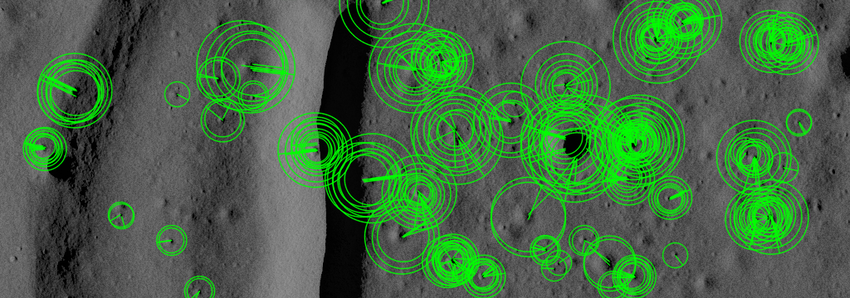
\includegraphics[width=\hsize]{figuras/kpts.png}
  \legend{Os círculos estão centrados nos pontos chaves que representam; a orientação é indicada com a linha que parte do ponto chave em direção ao círculo que o representa; e o raio do círculo é proporcional a redução de necessária da imagem para sua obtenção.}
  \source{Adaptado de \citeauthoronline{Ciarambino2016} (\citeyear{Ciarambino2016})}
\end{figure}

% Quais são os tipos de descritores disponíveis?
A descrição é a aplicação de alguma função nas vizinhanças de um pontos chave previamente detectado e resulta na preservação das características invariantes do ponto. Descritores são desenvolvidos para estar aptos a verificação de semelhança segundo alguma técnica de busca de dados ou cálculo de distâncias entre pontos no espaço de descrição. Entre as abordagens mais comuns de desenvolvimento de descritores estão as abordagens baseadas em histogramas de gradientes orientados \cite{SIFT1999,SURF}, computados em derivadas de imagens, e a descrição de por strings binárias \cite{AKAZE, ORB}, geralmente computados diretamente sobre as intensidades de \textit{pixels} nas imagens.

% O que é a correlação?
O estágio de correlação é o momento em que são comparadas as descrições dos pontos obtidos em uma imagem com o conjunto de descritores de uma outra imagem, ou de um conjunto de descritores de diversas imagens, a fim de encontrar as melhores correspondências para cada ponto. A estratégia adotada de forma mais ampla, para toda a imagem, é significativamente razoável se não há qualquer conhecimento prévio de onde ou entre quais imagens as correspondências devem ocorrer. Embora seja relativamente mais cara do que as técnicas de rastreamento de pontos, que perfazem buscas em conjuntos limitados de pontos e imagens, mas só estão disponíveis quando há como especular qual é a relação entre o conjunto de imagens. Por sua vez, as técnicas de correlação são frequentemente adotadas para inicializar (ou restaurar) o rastreamento, em aplicações de estabilização de vídeo por exemplo, sendo assim ambas as técnicas complementares entre si.

Ainda no contexto de correlações é possível considerar se cada hipótese de combinação entre pares de pontos precisa ser avaliada (abordagem de força bruta) ou se é possível explorar o espaço de descrição para realizar buscas por vizinhos mais próximos. A varredura extensiva de listas de descritores pode ser considerada uma solução precisa, mas pouco escalável, pois o custo de comparação de $K$ pontos em uma lista com $M$ outros pontos implica em $K \times M$ operações. Dentre as soluções alternativas destacam-se o uso de estruturas de dados capazes de emular o espaço de $N$
dimensões de um descritor, permitindo assim que algoritmos de busca por vizinhos mais próximos aproximados sejam usados tendo em vista que alguns podem levar a um número de operações que é aproximadamente $K \times \log{N}$.

\begin{figure}[!h]{15cm}
  \caption{Exemplo de correlação} \label{match}
  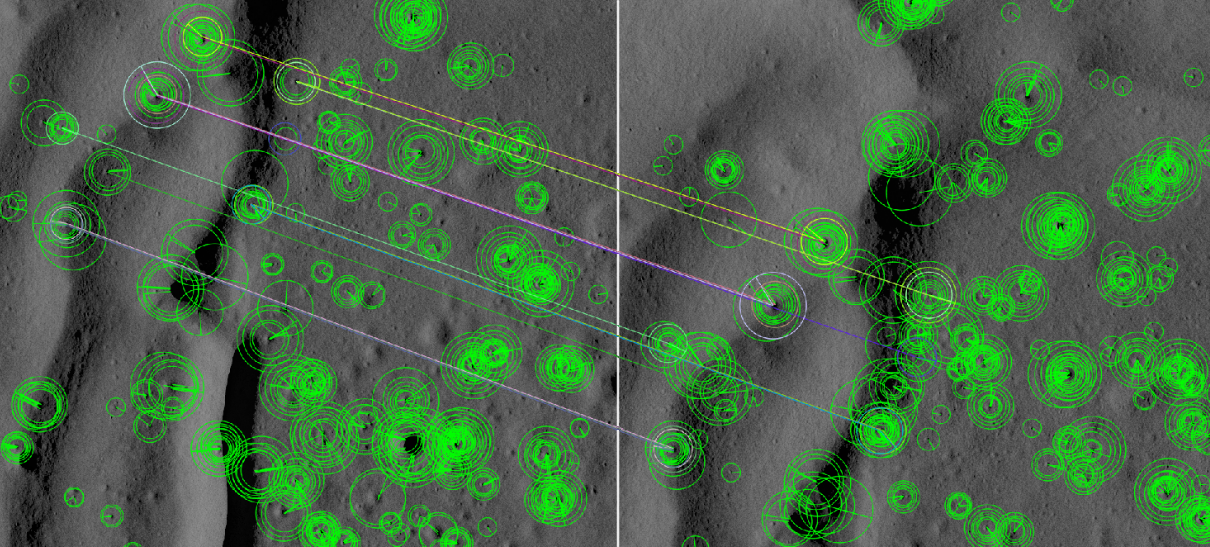
\includegraphics[width=\hsize]{figuras/match.png}
  \legend{Linhas em cores distintas indicam diferentes feições correlatas entre a imagem da esquerda e a da direita.}
  \source{Adaptado de \citeauthoronline{Ciarambino2016} (\citeyear{Ciarambino2016})}
\end{figure}

% Por que se adota a verificação geométrica?
Em ambos os casos de correlação a resposta para todos os pontos não é necessariamente o melhor resultado. Há que ser considerado que muitas correlações encontradas entre pares de pontos poderiam ser eliminadas por um limiar de distância. Estabelecer esse limiar ainda é um problema quando temos diferentes espaços de descrição a considerar. Outra questão importante é que a ordem de disposição das imagens num par analisado pode gerar resultados distintos.
Algo aceitável em determinadas aplicações, como a busca por objetos, mas que deve ser evitado em aplicações como a costura de imagens. Por sua vez, esta diferença em ambos os sentidos pode ser explorada para que a verificação cruzada preserve apenas as melhores correlações, quando elas concordarem entre si. Isto é útil principalmente nas aplicações de costura de imagens. Conforme ilustrado na Figura \ref{match} as melhores correlações, restritas por verificação cruzada, oferecem bom entendimento do movimento relativo entre as imagens num par. Outras alternativas podem ser previstas para que pontos chave que parecem correlacionar bem com mais de um ponto sejam deixados de fora, evitando assim o problema de pontos em regiões que podem ser considerados padrões repetitivos.

A melhor receita para robustecer a solução, e evitar que a aquisição automática de correlatos gere impactos ao processamento, é restringi-la usando o conhecimento prévio de como as imagens se formaram. Neste sentido, entre dois quadros obtidos por uma câmera, podemos encontrar uma transformação projetiva que leve os pontos de uma imagem em outra. Ao analisar os resíduos do transporte de pontos pela transformada, quando comparados com seus pares indicados pelas correlações, é possível destacar os conjuntos de pontos que permanecem na solução (\textit{inliers}) dos conjunto de pontos tratados como erros grosseiros (\textit{outliers}). Isto é feito em conjunto com técnicas de iteração e análise de consenso, para que possa ser verificado o grau de confiabilidade da resposta.



\subsection{A biblioteca OpenCV}

% Quem desenvolveu o opencv?
Lançado por Gary Bradski em 1999, enquanto trabalhava na Intel Corporation, na esperança de acelerar o desenvolvimento da visão computacional e da inteligencia artificial ao criar e fornecer uma infraestrutura sólida para todos que trabalham na área. Esta biblioteca foi escrita em C inicialmente, e portada ao C++ depois da versão 2.4.

% Quais os motivadores de sua escolha?
Esta biblioteca é desenvolvida como software livre e utilizável em todos os principais sistemas operacionais \cite{OpenCV}. Em sua área de concentração ela é umas das soluções mais disponíveis na atualidade, com grande número de interfaces para desenvolvimento de aplicações (APIs), tendo compatibilidade com linguagens como o Python, o Java, o Javascript e o C\#, além da linguagem C++, na qual é desenvolvida. Estão disponíveis também interfaces para uso conjunto com aplicações como o MATLAB e o GNU Octave. 

Devido a sua difusão não é difícil obter apoio para estudos dos conceitos deste campo, pois há muitos exemplos e tutoriais didáticos, questões e respostas em fóruns especializados, além de livros, cursos e códigos de aplicações \textit{open source} que fazem uso ativo desta biblioteca. Sua documentação, embora rudimentar em alguns aspectos, está ligada aos diversos trabalhos acadêmicos em que se basearam, desde que disponibilizados diretamente por seus autores.

A OpenCV está dividida em módulos e estes podem ainda ser divididos entre: principais, que formam a base estável e completamente open source; e extras, onde encontramos códigos de contribuidores isolados, experimentais ou patenteados, mas que já fazem parte da biblioteca por sua grande contribuição para a evolução da área. Mesmo com alguns recursos patenteados a biblioteca pode ser utilizada para fins acadêmicos, estando vedada a distribuição de binários executáveis com tais recursos para outros fins. Os módulos principais das versões mais recentes são listados na Tabela \ref{modulos}.

% Como a biblioteca está dividida?
\begin{table}[!ht]{12cm}
  \caption{Módulos da OpenCV 4.5.5}\label{modulos}
  \hfill
  \begin{tabular}{r|l}
    \hline
      Módulo & Descrição \\
    \hline
      core & Funcionalidade central \\
      imgproc & Processamento de imagens \\
      imgcodecs & Leitura e escrita dos formatos de imagem  \\
      videoio & Leitura e escrita dos formatos de video \\
      highgui & interface gráfica de alto nível \\
      video & Analise de video \\
      calib3d & Calibração de câmera e reconstrução 3D \\
      features2d & estrutura de recursos 2D \\
      objdetect & Detecção de objetos \\
      dnn & rede neural profunda \\
      ml & aprendizado de máquina \\
      flann & Clustering e Pesquisa em Espaços Multidimensionais \\
      photo & Fotografia computacional \\
      stitching & costura de imagens \\
      gapi & Interface de gráficos \\
    \hline
  \end{tabular}
  \hfill
  %\legend{(-) indica nenhuma dependência externa.}
  \source{`O autor'.}
\end{table}

% O que pode ser investigado para contribuir com o e-foto? (Alternativas ao SIFT)
O módulo \textit{features2d} apresenta a maior parte dos recursos necessários para a realização do presente trabalho. Entre os algoritmos integrados encontram-se o 
SIFT\footnote{SIFT refere-se a \textit{Scale Invariant Feature Transform} e foi publicado por \citeauthoronline{SIFT1999} em \citeyear{SIFT1999}} 
que há mais de 20 anos possibilitou um salto na detecção de objetos baseada em feições pontuais. Diversos outros algoritmos mais atuais, como o
AKAZE\footnote{AKAZE refere-se a \textit{Accelerated-KAZE} e foi publicado por \citeauthoronline{AKAZE} em \citeyear{AKAZE}}, 
ORB\footnote{ORB refere-se a \textit{Oriented FAST and Rotated BRIEF} e foi publicado por \citeauthoronline{ORB} em \citeyear{ORB}} e 
SURF\footnote{SURF refere-se a \textit{Speeded Up Robust Features} e foi publicado por \citeauthoronline{SURF} em \citeyear{SURF}} 
que reivindicam melhorias específicas e surgem como alternativas a serem comparadas em diversos cenários.

Discutiremos no Capítulo \ref{chp:metod} alguns recursos estendidos que podem ser obtidos nos módulos \textit{xfeatures2d} e \textit{cudafeatures2d}. São também importantes para o produto final os módulos \textit{core}, \textit{imgproc} e \textit{calib3d}. Os módulos \textit{highgui} e \textit{stitching} contribuem significativamente para este estudo, mas não são adotados como parte do produto final. Todavia, são igualmente relevantes para estudos futuros, pela proximidade com o assunto de fotogrametria, os módulos extras 
\textit{ccalib} (padrões personalizados de calibração para reconstrução 3D),
\textit{optflow} (fluxo óptico), 
\textit{reg} (registro de imagens), 
\textit{rgbd} (processamento com sensores de profundidade), 
\textit{sfm} (estruturação por movimento),
\textit{stereo} (correspondência densa),
\textit{structured\_light} (processamento de luz estruturada),
\textit{surface\_matching} (correlação de superfícies) e
\textit{tracking} (rastreamento).

% Os resumos de métodos para descrição foram suprimidos da versão final, pois eram muito breves, deste modo, cabe ao leitor do volume buscar mais informações nas referências deste trabalho.

%\subsubsection{SIFT}

%Apresentado em 1999 por David Lowe este algorítimo de detecção e descrição de feições que se utiliza de uma nova classe de feições que são invariantes a escala, translação, rotação , parcialmente invariantes a mudanças de iluminação e a projeções 3D e afim. E as feições são detectadas ao submeter as imagens em diferentes escalas e procurarmos os máximos locais utilizando a Diferença de Gaussiana \cite{SIFT1999}.

%\subsubsection{SURF}

%Mais recentemente o algorítimo SURF (Speeded Up Robust Features) apresenta um novo mecanismo de detecção e descrição de feições que são invariantes a escala e rotação,e promete se aproximar ou até performar melhor que seus antecessores. Ele depende da escala espacial gaussiana ao analisar as imagens, mas se baseia no uso da determinante da matriz Hessiana \cite{SURF}.

%\subsubsection{AKAZE}

%O algorítimo AKAZE (Accelerated-KAZE) foi apresentado em 2013 por P. F. Alcantrilla et al, e se propôs a acelerar alguns de seus antecessores, utilizando de exemplo o algoritimo KAZE que foi apresentado em 2012 pelos mesmos autores, que como ele se utilizam de filtragem de difusões não lineares. E para tal é apresentado o FED (Fast Explicit Diffusion) para ser uma alternativa a construção dos Espaços escaláveis não lineares (non-linear scale spaces) que em seus antecessores é um dos maiores fardos computacionais.

%\subsubsection{ORB}

%O algorítimo ORB (Oriented FAST and Rotated BRIEF) foi apresentado em 2011 por E. Rublee et al, e propõe ao combinar modificações no FAST (Features from Accelerated Segment Test) para detecção com os metodos de descrição do BRIEF (Binary Robust Independent Elementary Features) com direção normalizada, pois o descritos BRIEF é instável quanto a rotação, para criar este novo método de detecção e descrição de feições.
